\hypertarget{project-1-bqr-for-scalar-on-function-regression-with-heteroskedastic-data}{%
\section{Project 1: BQR for Scalar-on-Function Regression with
Heteroskedastic
Data}\label{project-1-bqr-for-scalar-on-function-regression-with-heteroskedastic-data}}

\hypertarget{background}{%
\subsection{Background}\label{background}}

\begin{frame}{General Introduction}
\protect\hypertarget{general-introduction}{}
\begin{itemize}
\tightlist
\item
  Quantile regression (QR) has gained popularity as a robust alternative
  to ordinary regression
\item
  QR is formulated as an optimization problem using a loss function
  \(\rho_\tau\), where \(\tau\) is the desired quantile
\item
  Bayesian Quantile Regression (BQR) offers the usual adventages of the
  Bayesian framework, like quantifying uncertainty
\item
  BQR is based on a likelihood function called the Asymmetric Laplace
  (AL) distribution whose kernel includes \(\rho_\tau\)
\end{itemize}
\end{frame}

\begin{frame}{GAL Distribution}
\protect\hypertarget{gal-distribution}{}
\begin{itemize}
\tightlist
\item
  AL turns out to be too restrictive
\item
  Yan and Kottas (2017) proposed the Generalized Asymmetric Laplace
  distribution (GAL)
\item
  It can be reparametrized with:

  \begin{itemize}
  \tightlist
  \item
    A location parameter \(\mu\)
  \item
    A scale parameter \(\sigma\)
  \item
    A shape parameter \(\gamma\)
  \end{itemize}
\item
  Closed forms for the pdf and cdf can be derived, but they are
  cumbersome
\end{itemize}
\end{frame}

\begin{frame}{Sampling from the posterior}
\protect\hypertarget{sampling-from-the-posterior}{}
\begin{itemize}
\tightlist
\item
  In Bayesian statistics, every parameter has a distribution
\item
  We sample from the distribution of \(\mu\), \(\sigma\) and \(\gamma\)
  using MCMC
\item
  In recent years, Hamiltonian Monte Carlo (HMC) has gained popularity
\item
  Implemented in the \lstinline!brms! library in R
\item
  Uses the same formula syntax as \lstinline!lme4!
\item
  Supports non-parametric methods through \lstinline!mgcv!
\end{itemize}
\end{frame}

\begin{frame}{Low dimensional ilustration of our problem}
\protect\hypertarget{low-dimensional-ilustration-of-our-problem}{}
\begin{itemize}
\tightlist
\item
  Consider data generated according to\\
  \begin{equation*}
   y_i = x_i^2 + \epsilon_i
   \end{equation*} where \(\epsilon_i \sim N(0, \exp(4x))\)
\end{itemize}

\begin{figure}
\centering
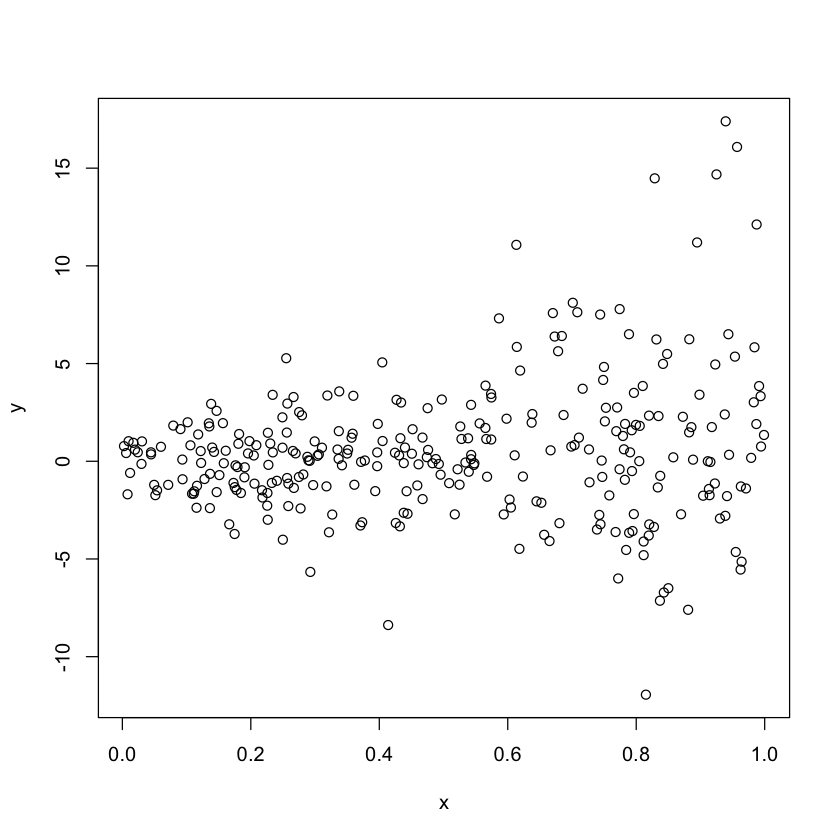
\includegraphics[width=0.5\textwidth,height=\textheight]{code_by_nico/functional/slides/htskdata.png}
\caption{heteroskedastic}
\end{figure}
\end{frame}

\begin{frame}
\begin{itemize}
\tightlist
\item
  Quantile regression should be able to handle this kind of
  heteroskedasticity
\item
  Turns out you have to be careful:

  \begin{lstlisting}
    model1 <- brm(y ~ s(x), family = 'GAL')
    model2 <- brm(y ~ s(x), sigma ~ s(x), family = 'GAL')
    \end{lstlisting}
\end{itemize}

\begin{figure}
\centering
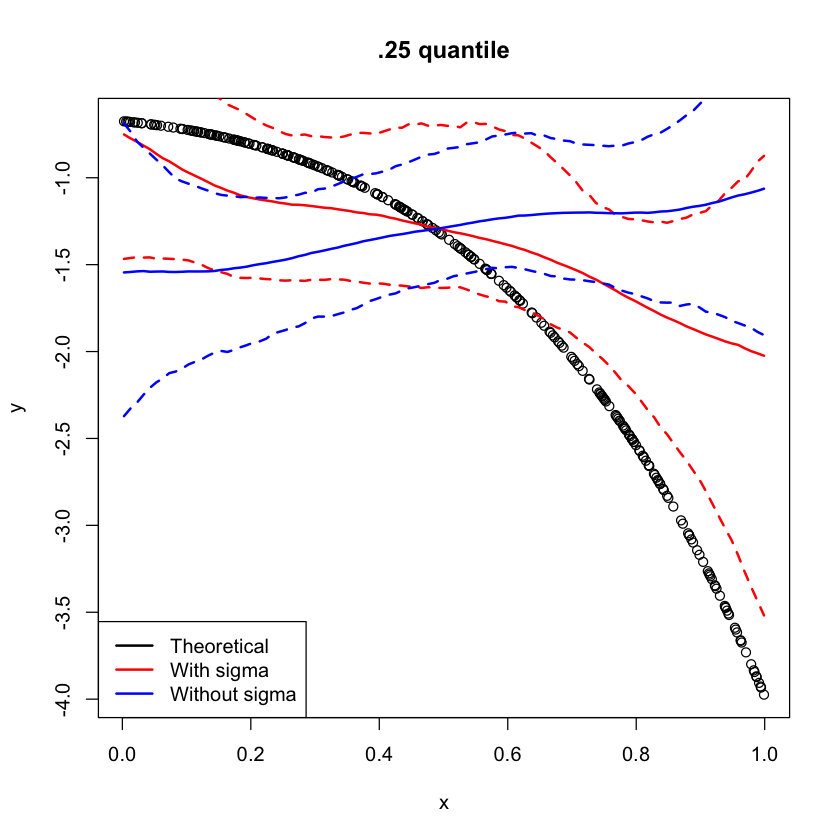
\includegraphics{code_by_nico/functional/slides/wandwo.png}
\caption{With and Without \(\sigma\)}
\end{figure}
\end{frame}
